L'aggiornamento del modello del dominio consiste in una rivisitazione del sistema di accesso, con l'utilizzo di two factor authentication con un codice Qr che viene fornito all'utente in fase di registrazione, per generare un codice numerico Totp, che verrà usato per effettuare l'accesso al sistema. In più RegistredUser e User sono diventate classi astratte, in quanto non é possibile istanziarle, ma solo estenderle. Poi é stata fatta una precisazione su Segnalazione, in quanto un Cliente può segnalare solo Codemonkeys e una Codemonkey può segnalare solo Clienti.\\
\linebreak

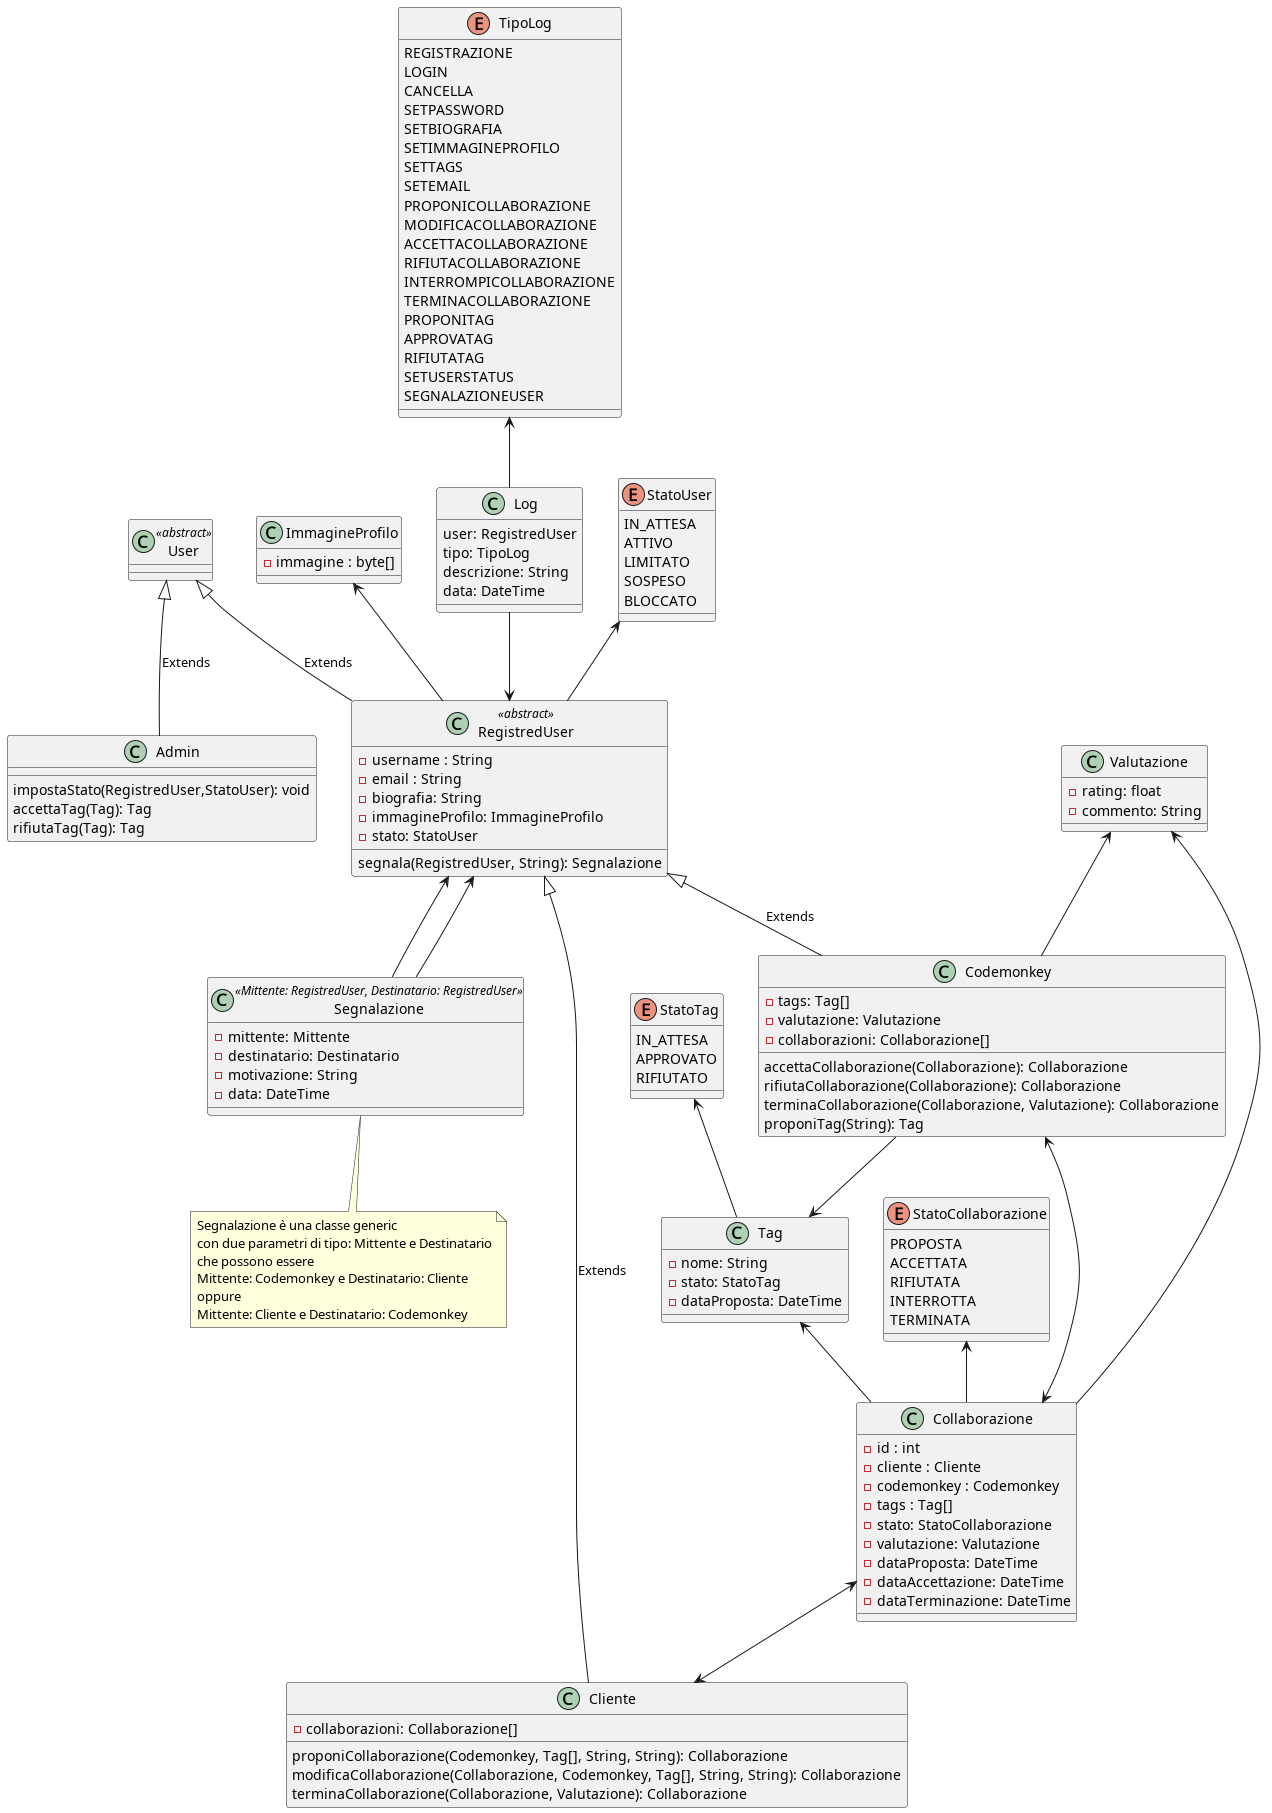
\includegraphics[width=1\textwidth]{assets/plantuml/modello_di_dettaglio_del_dominio.png}\\